%=======================================================================
%  Phase 2 Report -- CONDENSED (target: 10 pages)
%  Short companion to docs/phase2_report.tex (the full ~32 page paper).
%  Compile:  pdflatex phase2_report_short.tex   (run twice)
%=======================================================================
\documentclass[10pt,a4paper]{article}

\usepackage[margin=0.95in]{geometry}
\usepackage{amsmath,amssymb}
\usepackage{booktabs}
\usepackage{graphicx}
\usepackage{float}
\usepackage{caption}
\usepackage{algorithm}
\usepackage{algpseudocode}
\usepackage{tikz}
\usetikzlibrary{positioning,arrows.meta}
\usepackage[hidelinks,breaklinks=true]{hyperref}

\newcommand{\rs}{Rs.\,}
\newcommand{\code}[1]{\texttt{#1}}
\graphicspath{{figures/}}

\captionsetup{font=small, labelfont=bf}
\setlength{\parskip}{2pt}

\title{\vspace{-8mm}\textbf{Phase 2 Report (Condensed):\\
Cost-Aware Walk-Forward Validation, Probability Calibration and Risk
Management of an AI-Driven NSE BankNifty Options Trading System}}
\author{Anubhaw Raj \and Subham Singh \and Harsh Raj Sharma \and Nirban Das}
\date{\today}

\begin{document}
\maketitle
\vspace{-6mm}

\begin{abstract}
\small
Phase 1 built a momentum-driven Gradient Boosting classifier for NSE BankNifty
options and demonstrated it on a single trading day. This report condenses
Phase 2, in which that demonstration was turned into a measurement instrument
and then measured honestly. We (i) identify and repair a label-construction
defect in which the ``future price'' of a contract could be taken from a
\emph{different} contract, (ii) derive the full Indian options cost structure
and show it implies a break-even move of $1.0$--$3.0\%$ of premium per round
trip, (iii) build a Parquet feature store over roughly 1{,}200 trading days
(2020--2024) and a daily-retraining walk-forward engine with isotonic
probability calibration, threshold selection by simulated post-cost profit and
an abstention rule, and (iv) add a risk layer whose components we ablate on two
independent years. Full-year 2020 net profit and loss improves from
\rs$-349{,}791$ (4{,}706 trades) to \rs$-9{,}983$ (276 trades), a $35\times$
reduction, but the strategy remains unprofitable after costs: gross profit
turns slightly positive at a 15-minute horizon while charges stay near
\rs$57$ per trade, of which \rs$40$ is flat brokerage. Tight ($12\%$) intrabar
stops destroyed about \rs$116{,}000$ across 2020--2021 by harvesting
one-minute microstructure noise, and conviction sizing amplified a negative
expectancy. We conclude that the system sits at a trade-management noise floor
of \rs$-10{,}000$ to \rs$-16{,}000$ per year, and we state a falsifiable
hypothesis for the next phase: the training deadband ($0.1\%$) is an order of
magnitude below the cost hurdle ($\approx 1.5\%$), so the model is trained to
predict moves that cannot be traded profitably. Years 2022--2024 are an
untouched holdout. The full treatment, with derivations, code listings and
complete references, is in the companion Phase 2 paper.
\end{abstract}

\vspace{3mm}
\setcounter{tocdepth}{1}
\renewcommand{\contentsname}{\normalsize Contents}
{\small \tableofcontents}
\newpage

%=======================================================================
\section{Introduction}
%=======================================================================

Phase 1 \cite{phase1} established a pipeline over 1-minute BankNifty option,
spot and futures data: Black--Scholes--Merton features (moneyness, time to
expiry, implied volatility, Greeks) \cite{blackscholes}, a Gradient Boosting
binary classifier predicting whether an option's premium would be higher five
minutes later, and a two-state position machine trading a single at-the-money
(ATM) contract. It corrected two failure modes --- theta bias (fixed by moving
from regression to classification) and absolute-price overfitting (fixed by
replacing price levels with momentum) --- and reported $74.6\%$ accuracy on one
test day.

Four questions were left open, and they form the structure of this report:
\textbf{(1)} is the training label correct (Section~\ref{sec:label});
\textbf{(2)} does the edge survive brokerage, taxes and slippage
(Section~\ref{sec:costs}); \textbf{(3)} does it survive a full year, and a
second year (Sections~\ref{sec:infra} and~\ref{sec:results}); and
\textbf{(4)} does a score of $0.70$ actually mean $70\%$
(Section~\ref{sec:model}).

The scientific posture is deliberate. SEBI reports that $93\%$ of individual
traders in the equity derivatives segment lost money between FY22 and FY24
\cite{sebi}, so a claimed intraday edge should be assumed to be measurement
error until proven otherwise. Phase 2 optimised for trustworthy measurement,
not for a rising equity curve.

%=======================================================================
\section{Correctness: the label-leakage defect}\label{sec:label}
%=======================================================================

Phase 1 built the target by shifting the premium series $h$ rows forward on a
frame sorted by time:
$y_i = \mathbb{1}[\,p_{i+h} > p_i\,]$.
That frame stacks hundreds of contracts at every minute, so the row $h$
positions below a 32200\,CE quote generally belongs to a \emph{different}
contract --- often the opposite option type. The model was therefore trained on
a relation between two instruments, which is untradeable. It survived Phase 1
review because it still yielded high accuracy: premium ordering across strikes
is easy to predict from moneyness alone. This is the standard warning that in
financial machine learning the labelling step, not the model, is the usual
source of illusory performance \cite{lopezdeprado}.

The repair has three parts. First, group by contract before shifting:
\begin{equation}
y^{(s)}_t = \mathbb{1}\!\left[\, p^{(s)}_{t+h} > p^{(s)}_{t}(1+\delta) \,\right],
\end{equation}
so the comparison is always within one contract $s$. Second, a time-gap guard
invalidates any label whose realised time difference exceeds twice the horizon
($t^{(s)}_{+h} - t > 2h$), because illiquid contracts do not quote every
minute; such rows are dropped rather than imputed. Third, the deadband
$\delta$ requires the move to exceed a threshold, so the positive class means a
real move rather than a one-tick flicker. A unit test constructs two
interleaved contracts moving in opposite directions and asserts that each
contract's labels depend only on its own prices; it fails under the old rule
and passes under the new one.

%=======================================================================
\section{The transaction cost model}\label{sec:costs}
%=======================================================================

Let $q$ be the quantity traded, $P_b,P_s$ the buy and sell fills, and
$T_b=P_bq$, $T_s=P_sq$, $T=T_b+T_s$. The round-trip charge is
\begin{equation}
C = \underbrace{2B}_{\text{brokerage}} + \tau_{\text{stt}}T_s
  + \tau_{\text{txn}}T + \tau_{\text{sebi}}T + \tau_{\text{stamp}}T_b
  + \gamma\,(2B + \tau_{\text{txn}}T + \tau_{\text{sebi}}T),
\label{eq:cost}
\end{equation}
with $B=\rs 20$ flat per order, $\tau_{\text{stt}}=0.0625\%$ of sell premium,
$\tau_{\text{txn}}=0.05\%$, $\tau_{\text{sebi}}=0.0001\%$,
$\tau_{\text{stamp}}=0.003\%$ on the buy side and GST $\gamma=18\%$ on fees
\cite{zerodhacharges}. Slippage is applied to the fill itself rather than as a
lump sum, always against the trader: $P_b=P(1+\sigma_{\!f})$,
$P_s=P(1-\sigma_{\!f})$ with $\sigma_{\!f}=0.25\%$ per side.

Three structural facts drive the rest of the report: brokerage is \emph{flat},
so its share of cost is inversely proportional to position value; STT falls on
the sell side only; and GST multiplies the flat fee. The decision-relevant
quantity is therefore not the rupee charge but the \textbf{cost hurdle} --- the
percentage move needed to break even:
\begin{equation}
H(P,q) = \frac{C(P,P,q)}{Pq}\times 100 \;+\; 2\sigma_{\!f}\times 100 \quad [\%].
\label{eq:hurdle}
\end{equation}

\begin{table}[H]
\centering\small
\begin{tabular}{@{}rrrrr@{}}
\toprule
\textbf{Premium (\rs)} & \textbf{Lot} & \textbf{Charges (\rs)} &
\textbf{Charges (\%)} & \textbf{Hurdle $H$ (\%)}\\
\midrule
100 & 20 & 50.87 & 2.544 & \textbf{3.044}\\
300 & 20 & 58.22 & 0.970 & \textbf{1.470}\\
800 & 20 & 76.60 & 0.479 & \textbf{0.979}\\
300 & 25 & 60.98 & 0.813 & \textbf{1.313}\\
300 & 15 & 55.47 & 1.233 & \textbf{1.733}\\
\bottomrule
\end{tabular}
\caption{Break-even move per round trip from Equation~\eqref{eq:hurdle}
(slippage contributes a further $0.50\%$ in every row). For a \rs$300$ premium
at lot 20 the components are: brokerage \rs$40.00$, STT \rs$3.75$, exchange
\rs$6.00$, SEBI \rs$0.01$, stamp \rs$0.18$, GST \rs$8.28$. Cheap options are
disproportionately expensive because the flat fee dominates.}
\label{tab:hurdle}
\end{table}

Table~\ref{tab:hurdle} evaluates Equation~\eqref{eq:hurdle} for representative
premiums and lot sizes. Four consequences follow directly: avoid cheap
contracts; trade far less often;
prefer longer horizons, since $H$ is independent of the horizon while the
expected move is not; and amortise the flat fee over larger positions --- which
Section~\ref{sec:results} shows is only safe once expectancy is positive.
Lot size is not constant across the sample (BankNifty moved $20\to25\to15\to30$),
so it is stored as a step function keyed by effective date \cite{nsecircular}.

%=======================================================================
\section{Infrastructure: feature store and walk-forward engine}\label{sec:infra}
%=======================================================================

\paragraph{Architecture.} The data feed and the broker are interfaces rather
than concrete classes, so one signal, risk and execution path serves a
historical replay, a paper broker on live data, and a live broker
(Figure~\ref{fig:arch}). Promoting the validated system to live trading
therefore changes configuration, not strategy code, and removes the usual
rewrite step in which discrepancies appear between the backtested strategy and
the traded one.

\begin{figure}[H]
\centering
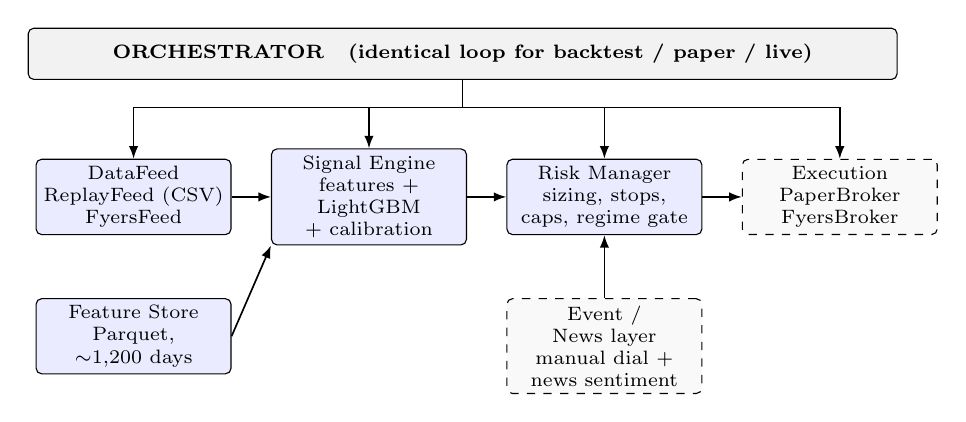
\begin{tikzpicture}[
  node distance=6mm and 5mm,
  box/.style={draw, rounded corners=2pt, align=center, minimum height=9mm,
              font=\scriptsize, inner sep=2.5pt, text width=23mm},
  done/.style={box, fill=blue!8},
  todo/.style={box, fill=gray!5, dashed},
  wide/.style={draw, rounded corners=2pt, align=center,
               font=\scriptsize\bfseries, minimum height=6.5mm,
               text width=108mm, fill=black!5},
  ar/.style={-{Latex[length=1.6mm]}, semithick}
]
\node[wide] (orch) {ORCHESTRATOR \; (identical loop for backtest / paper / live)};
\node[done, below=10mm of orch.south west, anchor=north west, xshift=1mm] (feed)
  {DataFeed\\ ReplayFeed (CSV)\\ FyersFeed};
\node[done, right=of feed] (sig)
  {Signal Engine\\ features + LightGBM\\ + calibration};
\node[done, right=of sig] (risk)
  {Risk Manager\\ sizing, stops,\\ caps, regime gate};
\node[todo, right=of risk] (exec)
  {Execution\\ PaperBroker\\ FyersBroker};
\node[todo, below=8mm of risk] (evt)
  {Event / News layer\\ manual dial +\\ news sentiment};
\node[done, below=8mm of feed] (store)
  {Feature Store\\ Parquet, $\sim$1{,}200 days};
\draw[ar] (orch.south) -- ++(0,-3.5mm) -| (feed.north);
\draw[ar] (orch.south) -- ++(0,-3.5mm) -| (sig.north);
\draw[ar] (orch.south) -- ++(0,-3.5mm) -| (risk.north);
\draw[ar] (orch.south) -- ++(0,-3.5mm) -| (exec.north);
\draw[ar] (store.east) -- (sig.south west);
\draw[ar] (evt.north) -- (risk.south);
\draw[ar] (feed.east) -- (sig.west);
\draw[ar] (sig.east) -- (risk.west);
\draw[ar] (risk.east) -- (exec.west);
\end{tikzpicture}
\caption{Target architecture. Shaded blocks are implemented and validated in
Phase 2; dashed blocks are specified and scheduled for the phases listed in
Section~\ref{sec:next}.}
\label{fig:arch}
\end{figure}

\paragraph{Feature store.} Implied volatility must be inverted numerically per
row, which made repeated experimentation infeasible. Each trading day is therefore processed once and
persisted as a columnar Parquet file; roughly 1{,}200 BankNifty days
(2020-01-01 to 2024-10-31) were built at about $0.8$\,s/day, after which a
full-year experiment costs minutes rather than hours.

\paragraph{Walk-forward evaluation.} This follows standard walk-forward
analysis \cite{pardo}: a sliding window of
$W=10$ days is split into a fit block and a calibration block, the next unseen
day is traded, and the window advances by one day --- about 240 iterations per
year (Algorithm~\ref{alg:wf}). Every quantity used to decide on day $d_k$ ---
model parameters, calibration map, entry threshold and the decision to trade at
all --- derives only from $\{d_{k-W},\dots,d_{k-1}\}$.

\begin{algorithm}[H]
\small
\caption{Walk-forward evaluation with calibration, threshold search and abstention}
\label{alg:wf}
\begin{algorithmic}[1]
\For{$k = W+1$ \textbf{to} $N$}
  \State $\mathcal{F} \gets$ first $W-c$ days before $d_k$;\quad
         $\mathcal{C} \gets$ last $c$ days before $d_k$ \Comment{$W=10$, $c=2$}
  \State build per-contract labels; fit LightGBM on $\mathcal{F}$
  \State fit isotonic calibrator on $\mathcal{C}$ (unseen by the fit)
  \State $\alpha^{\star},\Pi^{\star} \gets \arg\max_{\alpha}$ simulated
         \emph{post-cost} net profit on $\mathcal{C}$
  \If{$\Pi^{\star} \le 0$} \textbf{skip} day $d_k$
  \Else{} trade $d_k$ (ATM CE and PE state machines) at $\alpha^{\star}$ with the risk layer
  \EndIf
\EndFor
\end{algorithmic}
\end{algorithm}

\paragraph{Features.} Phase 1 described the contract; Phase 2 adds who is
trading it (Table~\ref{tab:features}). Scale-dependent inputs enter as rolling
z-scores rather than levels --- the Phase 1 lesson about absolute prices
generalised --- and time of day is encoded as $(\sin,\cos)$ of the session
fraction so that the two volatile session edges are not placed maximally far
apart.

\begin{table}[H]
\centering\small
\begin{tabular}{@{}lp{11.4cm}@{}}
\toprule
\textbf{Group} & \textbf{Features}\\
\midrule
Contract state (Phase 1) & moneyness, TTE, IV, delta, gamma, theta, vega\\
Momentum (Phase 1) & option and spot returns over 1 and 5 minutes\\
Contract flow & OI change 1m/5m, volume z-score, IV z-score\\
Chain-wide & put/call ratio (OI and volume), IV skew (PE$-$CE)\\
Futures & basis \%, futures returns 1m/5m, futures OI change, VWAP distance\\
Regime, calendar & realised volatility 15m/60m, minutes since open,
$\sin$/$\cos$ time of day, day of week\\
\bottomrule
\end{tabular}
\caption{The 30 model inputs. Warm-up \code{NaN}s are passed to the model
rather than dropped or imputed.}
\label{tab:features}
\end{table}

%=======================================================================
\section{Model, calibration and decision rules}\label{sec:model}
%=======================================================================

\paragraph{LightGBM.} With a model refitted for every test day --- over a
thousand fits per experiment --- training time is a design constraint. LightGBM
\cite{lightgbm} provides histogram binning, leaf-wise growth and up to a
$20\times$ speed-up at comparable accuracy, and it learns a default direction
for missing values, so rows with undefined rolling features (the opening
minutes, which are also the most volatile) still contribute. The objective is
log-loss, whose gradient under the logistic link is exactly $y_i-p_i$.

\paragraph{Calibration.} Boosted ensembles push scores towards the extremes, so
a raw $0.70$ may correspond to an empirical frequency near $0.55$
\cite{sklearncalib}. This matters because every downstream decision is a
threshold on that score. We therefore fit isotonic regression \cite{zadrozny}
on the calibration block,
$\min_{g \uparrow} \sum_i (y_i - g(\hat{s}_i))^2$,
solved by the Pool Adjacent Violators Algorithm. Being monotone, the map cannot
change the ranking and therefore cannot change AUC; it changes only what the
number means, which is the part the trading logic consumes.

\paragraph{Thresholds and abstention.} Expected net profit per trade is
$\mathbb{E}[\text{net}] = pW - (1-p)L - C$.
Accuracy implicitly sets the boundary at $p=0.5$, which is optimal only when
$W=L$ and $C=0$; with $C\approx\rs 57$ and $W\approx L$ it is guaranteed to
lose. We therefore replay each candidate threshold
$\alpha\in\{0.65,0.70,0.75,0.80\}$ through the complete stack --- state
machine, risk layer, costs --- on the calibration days and keep the most
profitable, with ties going to the higher threshold. If even the best threshold
loses money there, the system does not trade the next day at all. In the final
configuration it abstains on about $71\%$ of candidate days, which we treat as
a result rather than a defect: trading carries an unconditional cost and a
conditional benefit.

%=======================================================================
\section{The risk layer}\label{sec:risk}
%=======================================================================

The risk manager sits between signal and execution and can only reduce
activity. Entry gates: at most 4 trades per contract per day; a \rs$3{,}000$
daily loss kill-switch; no entry in the first 5 minutes or after 15:00; and a
realised-volatility band ($\text{rv}_{15}\in[0.02,0.30]$) excluding both dead
markets, where the hurdle cannot be cleared, and panic markets, where slippage
grows faster than the opportunity. Sizing uses a conviction ladder,
$n = \min(n_{\text{base}} + \lfloor (p-\alpha^{\star})/\kappa \rfloor,
n_{\max})$, subject to a premium cap. Exits race in order of conservatism:
intrabar stop, intrabar target, signal reversal ($p<0.45$), time limit, end of
day. With OHLC data the intrabar path is unknown, so when a bar spans both the
stop and the target we assume the stop was hit first.

\paragraph{Why a tight stop is a tax on noise.} A stop converts an unrealised
excursion into a realised loss, which helps only if the excursion is
information. Roll's result \cite{roll} shows that observed prices bounce
between bid and ask even when the efficient price is unchanged, inducing
negative serial covariance in price changes. A one-minute bar's low is thus
partly the bid side of a bouncing quote, not a price the market ``went to''.
For an ATM option with $\Delta\approx0.5$, a $12\%$ adverse excursion
corresponds to only a $0.1$--$0.2\%$ index move, which occurs many times per
session, so such a stop fires on ordinary noise and pays a full round trip each
time. Section~\ref{sec:results} quantifies the damage.

%=======================================================================
\section{Results}\label{sec:results}
%=======================================================================

All experiments use 2020 and 2021; \textbf{2022--2024 have never been
evaluated} and are reserved for a single confirmatory run.

\begin{table}[H]
\centering\small
\begin{tabular}{@{}lrrrrrr@{}}
\toprule
\textbf{Configuration (full-year 2020)} & \textbf{Trades} & \textbf{Gross} &
\textbf{Charges} & \textbf{Net} & \textbf{PF} & \textbf{Sharpe}\\
\midrule
Phase 2 baseline ($h=5$, fixed $0.70$, no risk layer)
  & 4{,}706 & $-72{,}379$ & $277{,}412$ & $-349{,}791$ & $0.70$ & $-7.58$\\
+ calibration, auto threshold, abstention ($h=5$)
  & 470 & $+5{,}225$ & $27{,}474$ & $-22{,}250$ & $0.79$ & $-2.60$\\
\textbf{+ horizon 15\,min}
  & \textbf{276} & $\mathbf{+5{,}710}$ & $\mathbf{15{,}693}$ &
  $\mathbf{-9{,}983}$ & $\mathbf{0.85}$ & $\mathbf{-1.82}$\\
+ horizon 30\,min
  & 236 & $-18{,}335$ & $13{,}936$ & $-32{,}271$ & $0.66$ & $-4.08$\\
\bottomrule
\end{tabular}
\caption{Cumulative effect of the Phase 2 work on one year of data (rupees,
net of all costs). Gross profit turns positive once the system stops trading
indiscriminately. At $h=30$ the average loss grows to \rs$805$ against an
average win of \rs$532$, indicating that beyond 15 minutes exit management
matters more than horizon.}
\label{tab:progress}
\end{table}

In Table~\ref{tab:progress} the baseline decomposition is the informative part:
gross is $\approx-\rs 15$ per trade --- statistically indistinguishable from
zero edge --- while charges are \rs$59$ per trade. The strategy was not losing
because its predictions were poor; it was losing because it traded roughly
twenty times a day. Figure~\ref{fig:equity} contrasts the two equity curves,
and Tables~\ref{tab:ablation} and~\ref{tab:exits} isolate what the risk layer
contributed.

\begin{figure}[H]
\centering
\begin{minipage}{0.49\textwidth}
\centering
\includegraphics[width=\textwidth]{fig01_baseline_equity.png}
\end{minipage}\hfill
\begin{minipage}{0.49\textwidth}
\centering
\includegraphics[width=\textwidth]{fig02_h15_equity.png}
\end{minipage}
\caption{Full-year 2020 net equity. \textbf{Left:} the Phase 2 baseline
($-\rs349{,}791$); the smooth monotone decline is the signature of a
cost-dominated strategy. \textbf{Right:} the best configuration
($h=15$\,min, $-\rs9{,}983$); flat stretches are days the abstention rule
declined to trade.}
\label{fig:equity}
\end{figure}

\begin{table}[H]
\centering\small
\begin{tabular}{@{}lrrrr@{}}
\toprule
\textbf{Configuration ($h=15$\,min)} & \textbf{2020 net} & \textbf{2021 net} &
\textbf{2020 trades} & \textbf{2021 trades}\\
\midrule
No risk layer (reference)                    & $-9{,}983$  & ---         & 276 & ---\\
$12\%$ stop, $\le 3$ lots                    & $-39{,}734$ & $-16{,}863$ & 144 & 167\\
$30\%$ stop, $\le 3$ lots                    & $-18{,}728$ & $-11{,}405$ & 91  & 99\\
$30\%$ stop, $1$ lot (final)                 & $-12{,}311$ & $-16{,}456$ & 97  & 103\\
\bottomrule
\end{tabular}
\caption{Risk-layer ablation on two independent years. The tight stop is
harmful in both; the remaining variants differ by less than the year-to-year
variation and the sign of the difference flips between years.}
\label{tab:ablation}
\end{table}

\begin{table}[H]
\centering\small
\begin{tabular}{@{}lrrrr@{}}
\toprule
& \multicolumn{2}{c}{\textbf{2020}} & \multicolumn{2}{c}{\textbf{2021}}\\
\cmidrule(lr){2-3}\cmidrule(lr){4-5}
\textbf{Exit reason ($12\%$ stop)} & Count & Net (\rs) & Count & Net (\rs)\\
\midrule
Signal reversal & 55 & $+8{,}083$ & 90 & $+23{,}067$\\
Target hit      & 10 & $+15{,}863$ & 8 & $+11{,}319$\\
Time limit      & 12 & $+1{,}389$ & 19 & $-85$\\
\textbf{Stop-loss} & \textbf{65} & $\mathbf{-64{,}738}$ & \textbf{50} &
$\mathbf{-51{,}164}$\\
\bottomrule
\end{tabular}
\caption{Net profit by exit reason. Every exit type other than the stop is net
positive in \emph{both} years; stop-outs alone account for \rs$115{,}902$ of
self-inflicted loss, at roughly \rs$1{,}000$ per occurrence. Widening the stop
to $30\%$ cut stop-outs from 65 to 9 in 2020.}
\label{tab:exits}
\end{table}

Position-size decomposition tells the same story for sizing: the 2-lot bucket
was the worst performer in three of four runs (2021: $-\rs20{,}789$ versus
$-\rs2{,}595$ for one lot). With $\mathbb{E}[\Pi_n]=n\mu$ and
$\operatorname{sd}[\Pi_n]=n\sigma$, scaling a negative $\mu$ multiplies the
loss and leaves $\mu/\sigma$ unchanged; sizing amplifies an edge but cannot
create one. The final configuration therefore sets $n_{\max}=1$ --- ``earn the
right to size up'' --- and yields, across two independent years: 97 and 103
trades, expectancy $-\rs126.9$ and $-\rs159.8$ per trade, profit factor $0.61$
and $0.50$, and maximum drawdown \rs$13{,}912$ and \rs$17{,}755$.

%=======================================================================
\section{Discussion}
%=======================================================================

\paragraph{Where the money goes.} At the best configuration, charges were
\rs$56.9$ per trade --- \rs$40$ of it flat brokerage --- against a gross edge of
$+\rs20.7$ per trade, giving $20.7-40.0-16.9=-\rs36.2$. Both remedies are
economic rather than algorithmic: raise the edge per trade, or amortise the
flat fee over a larger position (permissible only once expectancy is positive).

\paragraph{Noise floor.} Post-ablation variants differ by about
$\pm\rs5{,}000$ per year and the ranking flips between 2020 and 2021, so they
are no longer distinguishable from year-to-year variation. We characterise the
current state as a trade-management noise floor of \rs$-10{,}000$ to
\rs$-16{,}000$ per year and stopped tuning deliberately; further tuning would
fit the configuration to two specific years.

\paragraph{The deadband--hurdle mismatch.} The model is trained to answer
``will the premium be more than $0.1\%$ higher in 15 minutes?'' while the
system needs ``will it rise by $\approx1.5\%$ before my stop or time limit?''
These are different questions and the first is far easier, so a model with real
skill on it can still lose money. The remedy is to align the label with the
decision: set $\delta \approx H$, or adopt triple-barrier labelling
\cite{lopezdeprado}, where a sample is positive only if the profit target is
touched before the stop within the time limit. \textbf{Prediction:} headline
accuracy will fall and net expectancy per trade will rise. If it does not, our
account of why the strategy loses money is wrong and must be revised.

\paragraph{Threats to validity.} In descending order of concern:
(i) fifteen experiments were run and parameters chosen knowing 2020--2021
results, so the deflated Sharpe ratio \cite{deflatedsharpe} applies --- our
defence is procedural, namely the untouched 2022--2024 holdout;
(ii) fills are modelled from OHLC bars with a fixed $0.25\%$ slippage, not
observed from quotes;
(iii) the intrabar path is unknown and resolved pessimistically;
(iv) lot sizes come from secondary sources and must be verified circular by
circular before live use;
(v) purging and embargoing are not implemented, so labels may overlap the
fit/calibration boundary by up to $h$ minutes \cite{lopezdeprado};
(vi) results cover a single instrument and two years, one of which contains the
COVID-19 crash; and
(vii) the abstention rule estimates ``edge'' from only two days, so a
random-abstention control experiment is required.

%=======================================================================
\section{Conclusion and next steps}\label{sec:next}
%=======================================================================

Phase 1 produced a model; Phase 2 produced a measurement instrument and used it
honestly. It found a labelling defect that inflated accuracy, a cost structure
requiring a $1$--$3\%$ move per round trip, a raw edge indistinguishable from
zero at five minutes but slightly positive at fifteen, a stop rule that
destroyed \rs$116{,}000$ across two years, and a sizing rule that amplified a
negative expectancy. Removing these defects improved full-year 2020 net profit
from $-\rs349{,}791$ to $-\rs9{,}983$ while cutting trades from 4{,}706 to 276.

The strategy is not profitable, and we report that unchanged. The work is
nonetheless successful on three counts: each improvement is attributable to an
identified defect rather than to parameter search; every reported figure is net
of statutory charges and modelled slippage on data unseen at decision time; and
the work produced a specific, falsifiable hypothesis.

Next, in order: \textbf{(1)} label redesign via triple barriers at the cost
hurdle --- the highest-expected-value experiment, because a better model on a
misaligned target cannot help; \textbf{(2)} a controlled benchmark of logistic
regression, random forest, LightGBM, XGBoost \cite{xgboost}, CatBoost
\cite{catboost} and an LSTM under identical features, windows, costs and seeds,
selected on 2020--2021 and confirmed exactly once on the holdout, reporting the
deflated Sharpe ratio alongside the raw one, with probability averaging and a
model-disagreement abstention filter as extensions; \textbf{(3)} an event and
news risk layer producing a single $\text{event\_risk}\in[0,1]$ from headlines
plus a manual override, judged on drawdown reduction; \textbf{(4)} a simulated
live loop --- replay feed, paper broker, dashboard --- accepted only when it
reproduces the batch backtest for the same day; and \textbf{(5)} staged live
integration via the Fyers API \cite{fyers}. If the long-options edge remains
negative, the same infrastructure evaluates spreads or other strategies through
configuration rather than code, which is the lasting deliverable.

%=======================================================================
\begin{thebibliography}{99}
\small
%=======================================================================

\bibitem{phase1} A.~Raj, S.~Singh, H.~R.~Sharma and N.~Das,
\emph{Phase 1 Comprehensive Theory Paper}, May 2026. (Companion document.)

\bibitem{blackscholes} F.~Black and M.~Scholes, ``The Pricing of Options and
Corporate Liabilities,'' \emph{Journal of Political Economy}, 81(3), 1973.
\href{https://doi.org/10.1086/260062}{Link: Journal of Political Economy (DOI)}

\bibitem{lightgbm} G.~Ke et al., ``LightGBM: A Highly Efficient Gradient
Boosting Decision Tree,'' \emph{NeurIPS}, 2017.
\href{https://proceedings.neurips.cc/paper/2017/file/6449f44a102fde848669bdd9eb6b76fa-Paper.pdf}{Link: NeurIPS proceedings (PDF)}

\bibitem{xgboost} T.~Chen and C.~Guestrin, ``XGBoost: A Scalable Tree Boosting
System,'' \emph{ACM SIGKDD}, 2016.
\href{https://arxiv.org/abs/1603.02754}{Link: arXiv:1603.02754}

\bibitem{catboost} L.~Prokhorenkova et al., ``CatBoost: Unbiased Boosting with
Categorical Features,'' \emph{NeurIPS}, 2018.
\href{https://arxiv.org/pdf/1706.09516}{Link: arXiv:1706.09516 (PDF)}

\bibitem{zadrozny} B.~Zadrozny and C.~Elkan, ``Transforming Classifier Scores
into Accurate Multiclass Probability Estimates,'' \emph{ACM SIGKDD}, 2002.
\href{https://dl.acm.org/doi/10.1145/775047.775151}{Link: ACM Digital Library}

\bibitem{sklearncalib} scikit-learn developers, ``Probability Calibration.''
\href{https://scikit-learn.org/stable/modules/calibration.html}{Link: scikit-learn User Guide}

\bibitem{lopezdeprado} M.~L\'opez de Prado, \emph{Advances in Financial Machine
Learning}. Wiley, 2018. (Triple-barrier labelling, purged cross-validation.)

\bibitem{pardo} R.~E.~Pardo, ``Walk-Forward Analysis,'' in \emph{The Evaluation
and Optimization of Trading Strategies}, 2nd ed. Wiley, 2008.
\href{https://onlinelibrary.wiley.com/doi/abs/10.1002/9781119196969.ch11}{Link: Wiley Online Library}

\bibitem{deflatedsharpe} D.~H.~Bailey and M.~L\'opez de Prado, ``The Deflated
Sharpe Ratio,'' \emph{Journal of Portfolio Management}, 2014.
\href{https://papers.ssrn.com/sol3/papers.cfm?abstract_id=2460551}{Link: SSRN abstract 2460551}

\bibitem{roll} R.~Roll, ``A Simple Implicit Measure of the Effective Bid--Ask
Spread in an Efficient Market,'' \emph{Journal of Finance}, 39(4), 1984.
\href{https://www.bauer.uh.edu/rsusmel/phd/roll1984.pdf}{Link: University of Houston (PDF)}

\bibitem{sebi} Securities and Exchange Board of India, Press Release 22/2024,
September 2024.
\href{https://www.sebi.gov.in/media-and-notifications/press-releases/sep-2024/updated-sebi-study-reveals-93-of-individual-traders-incurred-losses-in-equity-fando-between-fy22-and-fy24-aggregate-losses-exceed-1-8-lakh-crores-over-three-years_86906.html}{Link: SEBI media and notifications}

\bibitem{zerodhacharges} Zerodha, ``Brokerage charges, fees and taxes.''
\href{https://zerodha.com/charges/}{Link: Zerodha charges}

\bibitem{nsecircular} National Stock Exchange of India, Circular
NSE/FAOP/56233, 31 March 2023.
\href{https://archives.nseindia.com/content/circulars/FAOP56233.pdf}{Link: NSE circular FAOP56233 (PDF)}

\bibitem{fyers} Fyers, \emph{fyers-apiv3} Python client.
\href{https://pypi.org/project/fyers-apiv3/}{Link: PyPI -- fyers-apiv3}

\end{thebibliography}

\end{document}
